\documentclass[sigplan,review]{acmart}
\usepackage[utf8]{inputenc}
%\usepackage{lmodern}
%\usepackage{uppunctlm}
\usepackage{amsmath}
\usepackage{array, caption, booktabs}
\usepackage{stmaryrd}
\usepackage{graphicx} % Required for inserting images
\usepackage{semantic}
\usepackage{mathtools}
\usepackage{float}
\usepackage{xspace}
%\usepackage{fancyvrb}
\usepackage{listings}
\usepackage{thmtools}
\usepackage{cleveref}
\usepackage{subcaption}

%\usepackage[
%backend=biber,
%style=numeric,
%sorting=ynt,
%maxcitenames=1,
%maxbibnames=99
%]{biblatex}
%\addbibresource{bibliography.bib}

\newcolumntype{L}{>{$}l<{$}} % left-oriented math column type
\newcolumntype{R}{>{$}r<{$}} % right-oriented math column type
\newcolumntype{C}{>{$}c<{$}} % center-oriented math column type

\newcommand{\lr}[1]{\langle #1 \rangle} % config macro: <#1>
\newcommand{\sub}[1]{\/\textsubscript{#1}} % subscript macro
\newcommand{\ltrans}[1]{\stackrel{#1}{\Rightarrow}} % labelled transition pil
\newcommand{\ltransn}[1]{\stackrel{#1}{\nRightarrow}} % labelled transition pil
\newcommand{\infeshort}[1]{\inference[{\normalsize(#1)}\;\;]} %formatting of \inference, when in a table side by side
\newcommand{\infelong}[1]{\inference[{\normalsize(#1)}\qquad]} %formatting of \inference, when on a single line
\newcommand{\define}{\stackrel{\text{def}}{=}} %def =
\newcommand{\encode}[1]{\llbracket #1 \rrbracket} %encoding brackets
\newcommand{\match}[1]{\{\mid #1 \mid\}} %encoding brackets
\newcommand{\child}{\textsf{child }} % 'child' stands out
\newcommand{\term}{$\lambda$-term\xspace} % lambda term
\newcommand{\OP}{\mathcal{O}} %family of operators
\newcommand{\OPc}{\hat{\mathcal{O}}} %cursorless family of operators
\newcommand{\OPcc}{\dot{\mathcal{O}}} %cursorless family of operators
\newcommand{\SORT}{\mathcal{S}} %set of sorts
\newcommand{\SORTc}{\hat{\mathcal{S}}} %set of cursorless sorts
\newcommand{\SORTcc}{\dot{\mathcal{S}}} %set of cursorless sorts
\newcommand{\VAR}{\mathcal{X}} %family of variables
\newcommand{\VARc}{\hat{\mathcal{X}}} %family of variables
\newcommand{\VARcc}{\dot{\mathcal{X}}} %family of variables
\newcommand{\AST}{\mathcal{A}[\VAR]} %family of asts
\newcommand{\ABT}[1]{\mathcal{B}[\VAR #1]} %family of abts
\newcommand{\ABTc}[1]{\hat{\mathcal{B}}[\VARc #1]} %family of cursorless abts
\newcommand{\ABTcc}[1]{\dot{\mathcal{B}}[\VARcc #1]} %family of cursorless abts
\newcommand{\alphac}{\rightarrow_\alpha} %alpha-conversion
\newcommand{\betar}{\rightarrow_\beta} %beta-reduction
\newcommand{\alphae}{\equiv_\alpha} %alpha-equivalence
\newcommand{\betae}{\equiv_\beta} %beta-equivalence
\newcommand{\stlc}{\ensuremath{\lambda_{->}}\xspace} %simply typed lambda calculus
\newcommand{\hole}[1]{\llparenthesis \ \rrparenthesis_#1} %hole, subscripted with a sort
\newcommand{\ctxhole}{[ \, \cdot \, ]} %context hole
\newcommand{\fix}{\text{fix}\xspace} %correct fix

\renewcommand{\vec}[1]{\overrightarrow{#1}}

\newcommand{\federeboks}[3]{
    \begin{figure}[H]
    \vspace{-2.9mm}
    \centering
    \fbox{%
        \footnotesize\renewcommand{\arraystretch}{1.25}
        \setlength{\tabcolsep} {4pt}
        \begin{tabular}{#1}
            \addlinespace[1.25ex]
            #2 \\
            \addlinespace[1.25ex]
        \end{tabular}
    }
    #3
    %\vspace{-2mm}
    \end{figure}
}

\newcommand{\skat}[1]{\ensuremath{\textbf{#1}}}
\newcommand{\Edt}{\skat{Edt}}
\newcommand{\Var}{\skat{Var}}
\newcommand{\Types}{\skat{Types}}

\newcommand{\pra}{\hookrightarrow}

\newcommand{\bs}{$\textbackslash$}

\lstdefinelanguage{elm}
{
    morekeywords={
            alias,
            as,
            case,
            else,
            exposing,
            if,
            import,
            in,
            let,
            module,
            of,
            port,
            then,
            type,
            where
        },
    sensitive=true, % Keywords are case-sensitive
    morecomment=[s]{\{-}{-\}}, % s is for start and end delimiter
    morecomment=[l]{--},
    morestring=[b]" % Defines that strings are enclosed in double quotes
}


\lstdefinestyle{inline}{
    columns=fullflexible,
    showspaces=false,
    showtabs=false,
    breaklines=true,
    showstringspaces=false,
    breakatwhitespace=true,
    escapeinside={(*@}{@*)},
    % commentstyle=\color{greencomments},
    % keywordstyle=\color{bluekeywords},
    % stringstyle=\color{redstrings},
    % numberstyle=\color{graynumbers},
    % numberstyle=\tiny\color{codegray},
    % backgroundcolor=\color{myinlinecolorback},
    basicstyle=\ttfamily\footnotesize,
    frame=single,
    frameround=tttt,
    tabsize=2,
    captionpos=b,
    numbers=none,
    % xleftmargin=2em,
}

\lstdefinestyle{examplestyle}{
    % backgroundcolor=\color{myexamplecolorback},
    % commentstyle=\color{codegreen},
    % keywordstyle=\color{magenta},
    % numberstyle=\tiny\color{codegray},
    % stringstyle=\color{codepurple},
    basicstyle=\ttfamily\footnotesize,
    breakatwhitespace=false,
    breaklines=true,
    captionpos=b,
    tabsize=2,
    frame=single,
    numbers=none,
    % xleftmargin=2em,
    frameround=tttt,
    % framexleftmargin=1.5em
}

\lstset{style=inline}

%%% Local Variables:
%%% mode: latex
%%% TeX-master: "Article"
%%% End:

\newcommand{\abt}{\textsf{abt}\xspace}
\newcommand{\ec}[1]{\ensuremath{\textsf{#1}}\xspace}
\newcommand{\rec}{\ec{rec}\,}
\newcommand{\chld}{\ec{child}\,}
\newcommand{\parnt}{\ec{parent}}
\newcommand{\nil}{\ec{nil}}

\AtBeginDocument{%
  \providecommand\BibTeX{{%
    Bib\TeX}}}

%% Rights management information.  This information is sent to you
%% when you complete the rights form.  These commands have SAMPLE
%% values in them; it is your responsibility as an author to replace
%% the commands and values with those provided to you when you
%% complete the rights form.
\setcopyright{acmcopyright}
\copyrightyear{2023}
\acmYear{2023}
\acmDOI{XXXXXXX.XXXXXXX}

\acmConference[PEPM 2025]{Make sure to enter the correct
  conference title from your rights confirmation emai}{January
  2025}{Denver, USA}

\acmPrice{15.00}
\acmISBN{978-1-4503-XXXX-X/18/06}


%%
%% Submission ID.
%% Use this when submitting an article to a sponsored event. You'll
%% receive a unique submission ID from the organizers
%% of the event, and this ID should be used as the parameter to this command.
%%\acmSubmissionID{123-A56-BU3}

%%
%% For managing citations, it is recommended to use bibliography
%% files in BibTeX format.
%%
%% You can then either use BibTeX with the ACM-Reference-Format style,
%% or BibLaTeX with the acmnumeric or acmauthoryear sytles, that include
%% support for advanced citation of software artefact from the
%% biblatex-software package, also separately available on CTAN.
%%
%% Look at the sample-*-biblatex.tex files for templates showcasing
%% the biblatex styles.
%%

%%
%% The majority of ACM publications use numbered citations and
%% references.  The command \citestyle{authoryear} switches to the
%% "author year" style.
%%
%% If you are preparing content for an event
%% sponsored by ACM SIGGRAPH, you must use the "author year" style of
%% citations and references.
%% Uncommenting
%% the next command will enable that style.
%%\citestyle{acmauthoryear}


%%
%% end of the preamble, start of the body of the document source.
\begin{document}

%%
%% The "title" command has an optional parameter,
%% allowing the author to define a "short title" to be used in page headers.
\title{A type-safe calculus for generating
  syntax-directed editors}

%%
%% The "author" command and its associated commands are used to define
%% the authors and their affiliations.
%% Of note is the shared affiliation of the first two authors, and the
%% "authornote" and "authornotemark" commands
%% used to denote shared contribution to the research.

%%\orcid{1234-5678-9012}

\author{Andreas Tor Mortensen}
\email{atmo20@student.aau.dk}


\author{Benjamin Bennetzen}
\email{bbenne20@student.aau.dk}


\author{Nikolaj Rossander Kristensen}
\email{nrkr20@student.aau.dk}

\author{Peter Buus Steffensen}
\authornotemark[1]
\email{psteff19@student.aau.dk
}

\affiliation{%
 \institution{Department of Computer Science at Aalborg University}
 \streetaddress{Selma Lagerlöfsvej 300}
 \city{Aalborg}
 \country{Denmark}
 \postcode{9220}
}

\author{Hans Huttel}
\email{hans.huttel@di.ku.dk}
\author{Sune Skaanning Engtorp}
\email{suneengtorp@live.dk}
\authornotemark[2]
\affiliation{%
 \institution{Department of Computer Science at University of Copenhagen}
 \streetaddress{Universitetsparken 1}
 \city{København}
 \country{Denmark}
 \postcode{2100}
}



%%
%% By default, the full list of authors will be used in the page
%% headers. Often, this list is too long, and will overlap
%% other information printed in the page headers. This command allows
%% the author to define a more concise list
%% of authors' names for this purpose.
\renewcommand{\shortauthors}{Bennetzen et al.}

\begin{abstract}
  
  Editor calculi make it possible to describe the actions of
  syntax-directed editing and provide guarantees of safety through
  their specialized type system: Well-typed editor scripts produce
  well-formed programs. So far, such calculi have been
  language-specific. In this paper we present a generalized editor
  calculus, which can be used to specify a specialized syntax-directed
  editor for any language, given its abstract syntax. Moreover we show
  how to implement an editor generator that allows one to generate an
  editor calculus-basedç syntax-directed editor from a language
  specification. The generalized editor calculus can be encoded into a
  simply typed lambda calculus, extended with pairs, booleans, pattern
  matching and fixed points. This implies a general type safety result
  that holdsfor any instantiation.
  
\end{abstract}

%%
%% The code below is generated by the tool at http://dl.acm.org/ccs.cfm.
%% Please copy and paste the code instead of the example below.
%%
\begin{CCSXML}
<ccs2012>
   <concept>
       <concept_id>10011007.10011006.10011050.10011023</concept_id>
       <concept_desc>Software and its engineering~Specialized application languages</concept_desc>
       <concept_significance>500</concept_significance>
       </concept>
   <concept>
       <concept_id>10003752.10010124.10010131</concept_id>
       <concept_desc>Theory of computation~Program semantics</concept_desc>
       <concept_significance>500</concept_significance>
       </concept>
   <concept>
       <concept_id>10003752.10010124.10010131.10010134</concept_id>
       <concept_desc>Theory of computation~Operational semantics</concept_desc>
       <concept_significance>500</concept_significance>
       </concept>
 </ccs2012>
\end{CCSXML}

\ccsdesc[500]{Software and its engineering~Specialized application languages}
\ccsdesc[500]{Theory of computation~Program semantics}
\ccsdesc[500]{Theory of computation~Operational semantics}


%%
%% Keywords. The author(s) should pick words that accurately describe
%% the work being presented. Separate the keywords with commas.
\keywords{Syntax-directed editor, Generalisation, lambda calculus}
%% A "teaser" image appears between the author and affiliation
%% information and the body of the document, and typically spans the
%% page.
%\begin{teaserfigure}
 % \includegraphics[width=\textwidth]{Images/windmill.jpg}
 % \caption{Seattle Mariners at Spring Training, 2010.}
%  \Description{Enjoying the baseball game from the third-base
%  seats. Ichiro Suzuki preparing to bat.}
%  \label{fig:teaser}
%\end{teaserfigure}

%\received{20 February 2007}
%\received[revised]{12 March 2009}
%\received[accepted]{5 June 2009}

%%
%% This command processes the author and affiliation and title
%% information and builds the first part of the formatted document.
\maketitle

\section{Introduction}

Syntax-directed editors aka projectional editors are specialized
editors that allow programmers to create programs directly using the
syntax of the programming language, thereby bypassing the need for
context-free parsing. A prominent early example of an editor of this
kind is that of the Cornell Program Synthesizer by Reps and Teitelbaum
\cite{10.1145/358746.358755}, designed with the PL/I language in mind.

Reps and Teitelbaum also demonstrated \cite{10.1145/390011.808247} how
one can generalize their original work to build a Synthesizer
Generator that will create a syntax-directed editor for any given
programming language, given a specification of its syntax in the form
of an attribute grammar. Around the same time, Donzeau-Gouge et
al. developed the Mentor programming environment
\cite{10.5555/800054.801990} that involved a command language, Mentol,
and allowed designers to specify language-specific specializations
using a specification language, Metal. More recently, in
\cite{10.1145/2997364.2997365} Voelker et al. introduce a notion of
grammar cells which is intended to be a formalism for defining textual
notations for syntax-directed editors. In
\cite{10.1145/3544548.3580785}, Beckmann et al. describe the
Sandblocks system that lets users automatically generate a
syntax-directed editor, given a description of the syntax of a given
language. The focus here is on that of usability of editors of this
kind.

Other recent developments introduce models of computation that
describe the workflow of syntax-directed editors and the correctness
properties that they must satisfy. The Hazelnut framework by Omar et
al. \cite{hazelnut} and the work by Godiksen et al. and
\cite{type_safe_structure_editor} introduce editor calculi that
describe the syntax and operational semantics of editing commands,
including how such commands can be combined. This line of work has
been tailored specifically towards functional programming: The edit
operations manipulate abstract syntax trees from an applied
$\lambda$-calculus.

A major advantage of this approach is that it is typed and that type
systems can be provably sound: The type system of the editor calculus
will then guarantee that if an editor term $E$ is well-typed, then $E$
will produce a well-formed program.

However, existing editor calculi do not account for context-sensitive
aspects of program syntax, and notably not the binding 
mechanisms that are prominent in abstract syntax.

Moreover, the work on editor calculi has so far been dependent on the
syntax of the programming language that the editor must
support. Whenever the programming language changes, the type soundness
results for the editor calculus have to be proved anew. An example of
this is the work by Andersen et al \cite{10.1145/3587216.3587221} on
extending the editor calculus of \cite{type_safe_structure_editor}
with let-declarations; the authors had to provide an entire new proof
of the soundness of the revised type system.

In this paper we propose a generalized editor calculus that deals with
these two issues and show how one can use this general framework to
devise an implementation that can generate an editor from a language
specification. 

Our calculus deals with binding mechanisms by using notions from
higher-order abstract syntax \cite{hoas}. Moreover, and importantly,
we show how to encode our generalized editor calculus into versions of
the simply-typed lambda calculus extended with pairs, booleans,
pattern matching and fixed-points. These fragments are all known to
have type systems with strong safety guarantees, and in this way we
obtain a general result on type safety that applies to any instance of
our generalized editor calculus.

\section{A Generalized Editor Calculus}\label{sec:general_editor}

We first present a generalization of the syntax-directed editor
calculus by \cite{type_safe_structure_editor}.

\subsection{Representing abstract syntax, cursors and holes}

Following Harper \cite{harper_foundations}, we assume that an abstract
syntax is given by a set of \emph{sorts} $\SORT$, an arity-indexed
family of \emph{operators} $\OP$ and a sort-indexed family of
variables $\VAR$.

The notions of \emph{cursors} and \emph{holes} are central to the idea
of an editor calculus. The cursor represents the point in an abstract
syntax tree where editing takes place, while holes represent the
places where subterms are yet to be filled in.

Whereas the calculus in \cite{type_safe_structure_editor} only has one
cursor and hole term and does not mention the notion of variable
binding, in the general case we need a cursor and hole operator for
every sort in the abstract syntax and to introduce binders.  With the
set of sorts $\SORT$, the extended family of operators $\OP$ and
family of variables $\VAR$ we define the sort-indexed family of
abstract binding trees (referred to as \abt in the following) $\ABT{}$
as the smallest family that satisfies the conditions of $\ABT{}$'s in
\cite{harper_foundations}.

We let $\hole{s}$ denote holes that can be replaced by terms of sort
$s$ and let $[e]$ note a cursor placed over the term $e$.

\begin{example}\label{ex:abstract_syntax}
Consider the following simple language of expressions with the binding
construct of local declarations.
\begin{align*}
  \text{Sort} && \text{Term} && \text{Operator} && \text{Arity} \\
        s & ::= & \text{let $x = e$ in $s$} && \text{let} && (e, e.s)s \\
        & | & e && \text{exp} && (e)s \\
  e & ::= & e_1 + e_2 && \text{plus} && (e,e)e \\
        & | & n && \text{num}[n] &&  ()e \\
        & | & x && \text{var}[x] && ()e
\end{align*}
 We can here represent
    \begin{equation*}
        \text{let $x=5$ in let $y=10$ in $x+y$}
    \end{equation*}
    as the ABT
    \begin{equation*}
        \text{let}(5;x.\text{let}(10;y.\text{exp}(\text{plus}(x;y))))
    \end{equation*} 
%
    We can extend this language with holes and cursors and get
    %
\begin{align*}
        \text{Sort} && \text{Term} && \text{Operator} && \text{Arity} \\
        s & ::= & [s] && \text{cursor}_s && (s)s \\
        & | & \hole{s} && \text{hole}_s && ()s \\
        e & ::= & [e] && \text{cursor}_e && (e)e \\
        & | & \hole{e} && \text{hole}_e && ()e
 \end{align*}
%
    With this extension the statement
    \begin{equation*}
        \text{let $x=[5]$ in $x+\hole{e}$}
    \end{equation*}
    is represented as the ABT
    \begin{equation*}
        \text{let}(\text{cursor}_e(5); x.\text{exp}(\text{plus}(x;\text{hole}_e)))    
    \end{equation*}
\end{example}

\subsection{The editor calculus}
Editor expressions $E \in \Edt$, where $\Edt$ is the sort of editor
expressions, describe the possible edit actions. The formation rules
are given below.
%
\begin{align*}
  E & ::= & \pi.E  \mid  \phi => E_1|E_2  \mid  E_1 \ggg E_2  \mid  \rec  \ x.E  \mid  x  \mid  \nil  \\
    \pi & ::= & \chld  \ n  \mid  \parnt   \mid  \{o\} \\
    \phi & ::= & \neg\phi  \mid  \phi_1 \wedge \phi_2  \mid  \phi_1 \vee \phi_2  \mid  @o  \mid  \Diamond o  \mid  \square o
\end{align*}
%
Evaluation of {\abt}'s, which \cite{type_safe_structure_editor}
introduces through an \textsf{eval} construct, is not included in our
generalized version. This omission is due to evaluation being entirely
dependent on the dynamics of the language in focus, and not the static
and structural properties the abstract syntax describes. To define the
concept of evaluation in a generalized manner, it would be necessary
to devise a formal and concise approach for specifying the semantics
of operators.

\begin{example}\label{ex:editor_calculus}
    We can define a version of the editor calculus for
    \cref{ex:abstract_syntax} by defining the set of operators $o$ ranges over. In this case we have that
    \begin{equation*}
        o \in \{ \text{let}, \text{exp}, \text{hole}_s, \text{plus}, \text{num}[n], \text{var}[x], \text{hole}_e \}
    \end{equation*}
    We can then write e.g. $(@\text{hole}_e =>
    \{\text{plus}\}.\nil |\nil )$. This expression would
    substitute the current tree encapsulated by the cursor with the
    $plus$ operator, if the cursor is at the operator
    $\text{hole}_e$. 
\end{example}

\subsection{Cursor contexts}

In editor expressions, we frequently refer to performing actions on,
or with, the \abt that is currently encapsulated by the cursor. To
support this notion we introduce cursor contexts $C$, inspired by the
zipper data structure by \cite{huet_zipper}, as a way to locate the
cursor in an ABT. Central to this idea is the cursor context
$\ctxhole$, or context hole, which specifies the subtree within which
the cursor must reside, either as the root, or one of the first
children.  For the full definition of cursor contexts, we refer to the
full version of the paper, or to \cite{type_safe_structure_editor}, as
they have a very similar construct. 

Although a cursor context accurately specifies the subtree where the
cursor must reside, it does not inherently guarantee the presence of
only one cursor within that subtree. Therefore, it becomes necessary
to introduce the concept of well-formed {\abt}'s. Informally, a
well-formed \abt is simply an \abt containing exactly one cursor. This
is guaranteed when an \abt can be interpreted as $C[a]$, meaning
the context $C$, where $\ctxhole$ is substituted with a tree $a$,
where the cursor-operator is either the root $a$, or one of the
children of the root. 


\subsection{Semantics}

In this section we present the transition systems and the general
forms of transition rules defining these systems, based on the
generalized syntax of the editor calculus previously presented.  

\subsubsection{Editor Expressions} \label{sec:Semantics}

Transitions for editor expressions are of the form
\[ \lr{E, a} \ltrans{\alpha} \lr{E', a'} \]
where the editor expression
$E \in \Edt$ is closed and the \abt $a \in \ABT{}$ is well-formed. The
labels of the transitions, $\alpha$, are the atomic prefix commands
$Apc$ and the silent transition $\epsilon$. The transition relation
$\Rightarrow$ is defined by the rules shown in
\cref{fig:editor_expression_rules}. These facilitate ways of composing
editor expressions together with conditions, sequential composition
and recursion. The means of traversing and modifying an \abt are
provided by the prefixed expression $\pi.E$, which evaluates $\pi$
before continuing with $E$. The conditional expression
$\phi => E_1|E_2$ reduces to $E_1$ if $\phi$ is satisfied and $E_2$
otherwise. The sequential expression $E_1 \ggg E_2$ evaluates $E_2$
only once $E_1$ has been reduced to $nil$. The recursive expression
$rec \ x.E$ binds the recursion variable $x$ in $E$, which can then be
used to recursively iterate an expression.

\federeboks{c}{
    \infeshort{Cond-1}
            {a |= \phi}
            {\lr{\phi => E_1 | E_2, C[a]} \ltrans{\epsilon} \lr{E_1, C[a]}}
    \\\\
    \infeshort{Cond-2}
        {a \nvDash \phi}
        {\lr{\phi => E_1 | E_2, C[a]} \ltrans{\epsilon} \lr{E_2, C[a]}}
    \\\\
    \infeshort{Seq}
        {\lr{E_1, a} \ltrans{\alpha} \lr{E_1',a'}}
        {\lr{E_1 \ggg E_2, a} \ltrans{\alpha} \lr{E_1' \ggg E_2,a'}}
    \\\\
    \infeshort{Seq-Trivial}
        {}
        {\lr{\nil  \ggg E_2, a} \ltrans{\epsilon} \lr{E_2,a}}    
    \\\\
    \infeshort{Recursion}
        {}
        {\lr{\rec  x.E,a} \ltrans{\epsilon} \lr{E[x:=rec \ x.E], a}}
    \\\\
    \infeshort{Context}
        {a \ltrans{\pi} a'}
        {\lr{\pi.E, C[a]} \ltrans{\pi} \lr{E, C[a']}}
}{\caption{Reduction rules for editor expressions}\label{fig:editor_expression_rules}}
.

\subsubsection{Substitution and cursor movement}

The labelled transition system for substitutions and cursor movement
is defined as $(\ABT{}, Apc, \Rightarrow)$. This system describes the
semantics of modifying the well-formed \abt $a$ encapsulated by the
cursor, by either substituting it with an operator or moving the
cursor up or down the tree. Transitions are therefore of the form $a
\ltrans{\pi} a'$, where $a, a' \in \ABT{}$ and $\pi \in Apc$. 

For substitution we define the transition rule for every label
$\{o\} \in Apc$, which substitutes the \abt currently encapsulated by
the cursor with an operator
$o(\Vec{x_1}.\hole{{s_1}}; \dots ; \Vec{x_n}.\hole{{s_n}})$ in which
the binders of the $i$'th argument of $o$ are $\Vec{x_i}$ and the sort
of the $i$'th argument is $s_i$. The general case of this rule is
shown in \cref{fig:substitution_rules}. The side-condition ensures
that we can only substitute operators of sort $s$ with {\abt}'s of
sort $s$.

\federeboks{c}{
    \infeshort{Ins}
        {}
        {[\hat{a}]  \ltrans{\{o\}} [o(\Vec{x_1}.\hole{{s_1}}; \dots ; \Vec{x_n}.\hole{{s_n}})]}
        $\begin{array}{l}
         \hat{a}, o \in \ABT{}_s % , \\ \text{ where $s$ is the sort of $o$}
        \end{array}$
}{\caption{General reduction rule for substitution with an
  operator with binders}\label{fig:substitution_rules}}

For cursor movement we define two transition rules "child  $i$" and
"parent" for every operator $o$ of arity $(\Vec{s_1}.s_1, \dots,$ $
\Vec{s_n}.s_n)s$ and for every $1 \leq i \leq n$. These rules, shown
in \cref{fig:cursor_movement_rules}, facilitate cursor movement from
the parent operator to child $i$ and from child $i$ back to the parent
operator, respectively.

\federeboks{c}{
    \infeshort{Child-i}
        {}
        {[\hat{o}(\Vec{x_1}.\hat{a}_1; \dots; \Vec{x_n}.\hat{a}_n)] \ltrans{\chld  \ i}} \\ 
        \quad \quad \quad \quad \quad $o(\Vec{x_1}.\hat{a}_1; \dots; \Vec{x_i}.[a_i]; \dots; \Vec{x_n}.\hat{a}_n)$
    \\\\
    \infeshort{Parent}
        {}
        {o(\Vec{x_1}.\hat{a}_1; \dots; \Vec{x_i}.[\hat{a}_i]; \dots; \Vec{x_n}.\hat{a}_n) \ltrans{\parnt }} \\
        \quad \quad \quad \quad \quad $[\hat{o}(\Vec{x_1}.\hat{a}_1; \dots; \Vec{x_n}.\hat{a}_n)]$
}{\caption{General reduction rules for cursor movement}\label{fig:cursor_movement_rules}}

\begin{example}\label{ex:substitution_rules}
    We now define the semantics of the editor calculus for our simple language. We do not show the transition rules for editor expressions, since these are equivalent to the ones presented in \cref{fig:editor_expression_rules}. 

    The transition system for cursor movement and substitution is defined with respect to the operators $o$ in our language. Based on the general form of substitution rules shown in \cref{fig:substitution_rules}, we define a specialized rule for substituting the tree encapsulated by the cursor for every operator $o$. A selection of these are shown in \cref{fig:example_substitution_rules}.
    \federeboks{c}{
        \infelong{let}
            {}
            {[\hat{a}]  \ltrans{\{\text{let}\}} [\text{let}(\hole{e};x.\hole{s})]}
            $\begin{array}{c}
             \hat{a} \in \ABT{}_s
            \end{array}$
        \\\\
        \infelong{plus}
            {}
            {[\hat{a}]  \ltrans{\{\text{plus}\}} [\text{plus}(\hole{e};\hole{e})]}
            $\begin{array}{c}
             \hat{a} \in \ABT{}_e 
            \end{array}$
        \\\\
        \infelong{var}
            {}
            {[\hat{a}]  \ltrans{\{\text{var} \ x\}} [x]}
            $\begin{array}{c}
             \hat{a} \in \ABT{}_e
            \end{array}$
    }{\caption{Selected reduction rules for substitution}\label{fig:example_substitution_rules}}
    Notice that in every rule we ensure that the substitution can only be performed if the \abt $\hat{a}$ is of the same sort as the operator. For example, given the configuration \[ \lr{\{let\}.nil, \text{let $x = [\hole{e}]$ in $x+x$}}\] we cannot substitute in a statement, as shown below.
    \begin{center}
    \begin{tabular}{c}
        \inference[\runa{Context}]
            {\inference[(let)]
                {}
                {[\hole{e}]  \ltransn{\{\text{let}\}}}
                $\begin{array}{c}
                    \hole{e} \notin \ABT{}_s
                \end{array}$
            }
            {\lr{\{\text{let}\}.\nil , \text{let $x = [\hole{e}]$ in $x+x$}} \ltransn{\{\text{let}\}}}
    \end{tabular}
    \end{center}
        
    Similarly, using the general form of cursor movement transition rules in \cref{fig:cursor_movement_rules}, we define specialized rules for every argument $i$ of every operator $o$. In \cref{fig:example_cursor_movement_rules} we show the parent and child rules for the let operator specifically. The transition rules for the remaining operators would be defined analogous to these.
    \federeboks{c}{
        \infelong{letc-1}
            {}
            {[\text{let}(a_1; x.a_2)] \ltrans{\chld  \ 1} \text{let}([a_1]; x.a_2)}
        \\\\
        \infelong{letc-2}
            {}
            {[\text{let}(a_1; x.a_2)] \ltrans{\chld  \ 2} \text{let}(a_1; x.[a_2])}
        \\\\
        \infelong{letp-1}
            {}
            {\text{let}([a_1]; x.a_2) \ltrans{\parnt } [\text{let}(a_1; x.a_2)]}
        \\\\
        \infelong{letp-2}
            {}
            {\text{let}(a_1; x.[a_2]) \ltrans{\parnt } [\text{let}(a_1; x.a_2)]}
    }{\caption{Reduction rules for cursor movement on the $let$ operator}\label{fig:example_cursor_movement_rules}}
\end{example}

\subsubsection{Conditions}
Finally, we define the satisfaction relation for conditions $\phi$ in
our editor calculus. The propositional connectives are defined as
expected in \cref{fig:satisfaction_relation_connectives}.

\federeboks{c}{
        \infeshort{Negation}
        {[\hat{a}] \nvDash \phi}
        {[\hat{a}] |= \neg \phi}
    \\\\
    \infeshort{Conjunction}
        {[\hat{a}] |= \phi_1 \quad [\hat{a}] |= \phi_2}
        {[\hat{a}] |= \phi_1 \wedge \phi_2}
    \\\\
    \infeshort{Disjunction-1}
        {[\hat{a}] |= \phi_1}
        {[\hat{a}] |= \phi_1 \vee \phi_2}
    \\\\
    \infeshort{Disjunction-2}
        {[\hat{a}] |= \phi_2}
        {[\hat{a}] |= \phi_1 \vee \phi_2}
}{\caption{Satisfaction relation for propositional connectives}\label{fig:satisfaction_relation_connectives}}

% \begin{figure}[h]
%   \centering
%   \begin{tabular}{lc}
%   \infeshort{Negation}
%         {[\hat{a}] \nvDash \phi}
%         {[\hat{a}] |= \neg \phi}
%     \\\\
%     \infeshort{Conjunction}
%         {[\hat{a}] |= \phi_1 \quad [\hat{a}] |= \phi_2}
%         {[\hat{a}] |= \phi_1 \wedge \phi_2}
%     \\\\
%     \infeshort{Disjunction-1}
%         {[\hat{a}] |= \phi_1}
%         {[\hat{a}] |= \phi_1 \vee \phi_2}
%     \\\\
%     \infeshort{Disjunction-2}
%         {[\hat{a}] |= \phi_2}
%     {[\hat{a}] |= \phi_1 \vee \phi_2}
%     \end{tabular}
%   \caption{Satisfaction relation for propositional connectives}
%   \label{fig:satisfaction_relation_connectives}
% \end{figure}

The general form of the satisfaction rules for the modalities $@o$,
$\Diamond o$ and $\square o$ are defined in
\cref{fig:satisfaction_relation_modal}.

\federeboks{c}{
    \infeshort{At-op}
        {}
        {[o(\Vec{x_1}.\hat{a}_1; \dots; \Vec{x_n}.\hat{a}_n)] |= @o }  
    \\\\
    \infeshort{Necessity}
        {[\hat{a}_1] |= \Diamond o \ \dots \ [\hat{a}_n] |= \Diamond o}
        {[o(\Vec{x_1}.\hat{a}_1; \dots; \Vec{x_n}.\hat{a}_n)] |=\square o}
    
    \\\\
    \infeshort{Possibly-i}
        {[\hat{a}_i] |= \Diamond o}
        {[o(\Vec{x_1}.\hat{a}_1; \dots; \Vec{x_i}.\hat{a}_i; \dots; \Vec{x_n}.\hat{a}_n)] |= \Diamond o}
    \\\\
    \infeshort{Possibly-trivial}
        {[\hat{a}] |= @o}
        {[\hat{a}] |= \Diamond o}
}{\caption{Satisfaction relation for modal operators}\label{fig:satisfaction_relation_modal}}
The modality $@o$ holds for an \abt $a$ if the cursor is at the root of
$a$ and the root is the operator $o$. 

The modality $\Diamond o$ is satisfied for $a$ when the operator $o$ is
anywhere within $a$. The modality
$\square o$ holds for $a$ when $o$ is found in every subtree of the
ABT encapsulated by the cursor. 

% \begin{example}\label{ex:modal_logic}
%     We finalize our specialized editor calculus from \cref{ex:substitution_rules}, by defining the satisfaction relation. The propositional connectives are defined as previously shown in \cref{fig:satisfaction_relation_connectives}. In \cref{fig:example_satisfaction_relation} we have shown the satisfaction rules for all modalities for the $plus$ operator. Rules for the remaining operators $o$ are defined accordingly.
%     \federeboks{c}{
%         \infeshort{At-plus}
%             {}
%             {[\text{plus}(\hat{a}_1;\hat{a}_2)]|= @\text{plus} }  
%         \\\\
%         \infeshort{Pos1-plus}
%             {[\hat{a}_1] |= \Diamond o}
%             {[\text{plus}(\hat{a}_1; \hat{a}_2)] |= \Diamond o}
%         \\\\
%         \infeshort{Nec-plus}
%             {[\hat{a}_1] |= \Diamond o \quad [\hat{a}_2] |= \Diamond o}
%             {[\text{plus}(\hat{a}_1;\hat{a}_2)] |=\square o}
%         \\\\
%         \infeshort{Pos2-plus}
%             {[\hat{a}_2] |= \Diamond o}
%             {[\text{plus}(\hat{a}_1; \hat{a}_2)] |= \Diamond o}
%     }{\caption{Satisfaction relation for modal operators on $plus$}\label{fig:example_satisfaction_relation}}
% \end{example}

\subsection{Guarantees from the original editor calculus}

The original editor calculus of \cite{type_safe_structure_editor} is
equipped with a type system that types configurations relative to a
path in the ast of the configuration; this path represents the
position of the cursor. Judgments are therefore of the form
$p, \Gamma_e \vdash \lr{E,a} : \textsf{ok}$, where $p$ is a path in
the ast $a$ and $\Gamma_e$ is a type environment.

The type system of the original calculus guarantees that a well-typed
configuration remains well-typed after a transition and that a
well-typed configuration will not get stuck. Here,
$(p,\Gamma_e)\downarrow_\alpha$ denotes that the path and the type
environment are updated because of the action $\alpha$. These
guarantees can be expressed as the following theorem.

\begin{theorem}[\cite{type_safe_structure_editor}]\label{thm:typesafe}
  If $p, \Gamma_e \vdash \lr{E,a} : \textsf{ok}$ then
  \begin{enumerate}
  \item if $\lr{E,a} \ltrans{\alpha} \lr{E',a'}$, then
    $(p,\Gamma_e)\downarrow_\alpha \, \vdash \lr{E',a'} : \textsf{ok}$
  
  \item $p, \Gamma_e \vdash \lr{E,a} \not\to \textsf{wrong}$
  \end{enumerate}
\end{theorem}

\section{Encoding the generalized editor calculus} \label{sec:encoding}


\subsection{A collection of lambda calculi}

To encode the abstract binding trees, the simply typed lambda calculus
suffices, so for an \abt $a$ its encoding $\encode{a}$ is a term in
$\stlc$.

In order to encode ABTs with cursors and expressions of the
generalized editor calculus, we extend \stlc with more constructs.

To represent contexts, we introduce pairs. To encode atomic prefix
commands we further extend the calculus with pattern matching
($\lambda_{->,p}$). Finally, to encode modal logic and editor
expressions recursion is needed in the form of the fixed point
operator ($\lambda_{->,p,\fix}$).

An overview of the calculus and the constructs necessary to encode
each part of it can be seen in \cref{tab:encoding_requirements}.

\begin{table*}
   \centering
   \begin{tabular}{| l | l |}
       \hline
       \textsf{Editor calculus} & \textsf{Encoding}\\
       \hline\hline
       \ Abstract Binding Trees & \ Simply typed lambda calculus with pairs, \stlc \\
       \hline
       \ Atomic Prefix Commands & \ \stlc with pattern matching $\lambda_{->,p}$\\
       \hline
       \ Modal Logic & \ \stlc with pattern matching and recursion, $\lambda_{->,p,\fix}$ \\
       \hline
       \ Editor Expressions & \ \stlc with pattern matching and recursion, $\lambda_{->,p,\fix}$ \\
       \hline 
   \end{tabular}
   \vspace{1mm}
   \caption{Editor calculus fragments and the lambda calculus fragments
     used for encoding them}
   \label{tab:encoding_requirements}
 \end{table*}

 All of the lambda calculi that we consider have a
 standard reduction semantics with reductions of the form $e \to
 e'$.

 Moreover, every calculus has a type systems with judgements of the
 form $\Gamma \vdash e : \tau$, where $\tau$ ranges over a set of
 types \Types\ given by
%
\[  \tau ::= \tau_s \mid \tau \to \tau \mid \tau \times \tau  \]
%
where $\tau_s$ is a type for each sort $s \in \mathcal{S}$ and $\tau
\to \tau$ and $\tau \times \tau$ are function and product types,
respectively, and $\Gamma$ is a type environment
 $\Gamma : \Var \pra \Types$. 

 The type systems all satisfy the subject
 reduction property.

 \begin{theorem}[Subject reduction]\label{thm:subred}
   If $\Gamma \vdash e : \tau$ and $e \to e'$, then $\Gamma \vdash e'
   : \tau$.
 \end{theorem}

 It is this result that ensures that our encoding will indeed provide
 a general result about type soundness for the generalized editor
 calculus.
 
\subsection{Abstract binding trees}

To encode abstract binding trees we only need to use the simply typed
lambda-calculus where we have term constants $o$ for every $o \in \OP$
excluding cursors, and the base types $s$ for every $s \in \SORT$.

Typing rules for operators can be seen on \cref{fig:abt_typing_rules},
where we can infer the type of an operator in the lambda-calculus by
its arity.  
\federeboks{C}{
    \infeshort{T-Operator}
        {o \in \OP \text{ and has arity } (\Vec{s_1}.s_1, \dots, \Vec{s_n}.s_n)s}
        {\Gamma |- o : (\Vec{s_1} -> s_1) -> \dots (\Vec{s_n} -> s_n) -> s}
}{
    \caption{Typing rules for operators.}
    \label{fig:abt_typing_rules}
}

With the operators added as term constants and sorts added as base
types, encoding ABTs is straightforward as we just have to curry the
operator $o$, encode the children $a_1, \dots, a_n$ and add
typings. This can be seen on \cref{fig:enc_abt}. 

\federeboks{C}{
    \encode{o(\Vec{x_1}.a_1, \dots , \Vec{x_n}.a_n)} = o \ (\lambda \Vec{x_1} : \Vec{s_1}.\encode{a_1}) \dots (\lambda \Vec{x_n} : \Vec{s_n}.\encode{a_n})
}{
    \caption{Encoding of abstract binding trees.}
    \label{fig:enc_abt}
}

\begin{example}\label{ex:enc_abt_example}
    We can now encode the operators in our small language. Following
    our singular rule for encoding {\abt}'s we get the resulting encoding
    seen on \cref{fig:enc_abt_example}, and the type for each operator
    on \cref{fig:abt_example_type}. 
    
    \federeboks{C C}{
        \encode{\text{plus}(a_1; a_2)} = \text{plus} \encode{a_1} \encode{a_2} 
        &
        \encode{\text{num}[n]} = \text{num}[n]
        \\\\
        \encode{\text{var}[x]} = \text{var}[x]
        &
        \encode{\text{hole}_e} = \text{hole}_e
        \\\\
        \encode{\text{exp}(a_1)} = \text{exp} \encode{a_1}
        &
        \encode{\text{hole}_s} = \text{hole}_s
        \\\\
        \multicolumn{2}{C}{
            \encode{\text{let}(a_1; x.a_2)} = \text{let} \ (\encode{a_1}) (\lambda x : e. \encode{a_2})
        }
    }{
        \caption{Encoding of operators.}
        \label{fig:enc_abt_example}
    }
    
    \federeboks{C C}{
        \text{plus} : e \to e \to e
        &
        \text{num}[n] : e
        \\\\
        \text{var}[x] : e
        &
        \text{hole}_e : e
        \\\\
        \text{exp} : e \to s
        &
        \text{hole}_s : s
        \\\\
        \multicolumn{2}{C}{
            \text{let} : e \to (e \to s) \to s
        }
    }{
        \caption{Types of the encoded operators.}
        \label{fig:abt_example_type}
    }
    
\end{example}

for example, if we were to encode the statement:
\begin{equation*}
        \text{let $x=[\hole{e}]$ in $x+5$}
    \end{equation*}
    it could be encoded as:
    \begin{align*} 
        \text{let} \ (\text{cursor}_e(\text{hole}_e)) \ (\lambda x . \text{plus} \ \text{var}[x] \ \text{num}[5])
  \end{align*}




\subsection{Cursor contexts}\label{sec:enc_cursor_contexts}

To represent ABTs with cursor contexts we introduce the pair construct similarly to \cite{types_programming_languages}.
%In \cref{fig:abt_cursor_syntactic_forms} we introduce the new syntactic forms which include the pair construct, first projection, second projection and the product type. 
%\federeboks{R C L l}{
%    \multicolumn{4}{c}{Terms}
%    \\
%    M & ::= &(M_1,M_2) & (pair) \\
%      & |   & M.1      & (first projection) \\
%      & |   & M.2      & (second projection)
%    \\\\
%    \multicolumn{4}{c}{Types}
%    \\
%    \tau & ::= & \tau_1 \times \tau_2 & (product type)
%}{\caption{Abstract syntax for representing cursor contexts as pairs.}\label{fig:abt_cursor_syntactic_forms}}


In \cref{fig:enc_abt_cursor} the encoding for cursor contexts can be seen. We can encode a cursor context $C[a]$ as a pair of two encoded trees the first being a regular \abt and the second being an \abt with a context hole $\ctxhole$, which we encode as an operator $\ctxhole$. We also introduce a type alias such that $\encode{C[a]}$ has type $Ctx = s \times s$.
\federeboks{C}{
    \encode{C[a]} = (\encode{a}, \encode{C}) \\
    \encode{\ctxhole} = \ctxhole
}{
    \caption{Encoding of cursor contexts.}
    \label{fig:enc_abt_cursor}
}

%\begin{example}
%    In \cref{ex:well_formed_trees} we saw that the expression.
%    \begin{equation*}
%        \text{let $x=[\hole{e}]$ in $x+5$}
%    \end{equation*}
%    is well-formed since it can be written as $C[\dot{e}]$ where
 %   \begin{align*}
 %       C &= \quad \text{let $x=\ctxhole$ in $x+5$} \\
  %      \dot{e}&= \quad [\hole{e}]
  %  \end{align*}
%    Encoding $C[\dot{e}]$ following the rules for encoding contexts and the rules for encoding abts in \cref{ex:enc_abt_example} yields the following encoding:
%    \begin{align*}
 %       & \encode{C[\dot{e}]} = \\ 
 %       & (\encode{\text{cursor}_e(\text{hole}_e)}, \encode{\text{let}([\cdot]; x.\text{plus}(\text{var}[x], \text{num}[5]))}) = \\ 
 %       & (\text{cursor}_e(\text{hole}_e), \text{let} \ [\cdot] \ (\lambda x . %\text{plus} \ \text{var}[x] \ \text{num}[5]))
 %   \end{align*}
    
%\end{example}

\subsection{Atomic prefix commands}

To encode the atomic prefix commands we further extend the lambda
calculus with pattern matching. The formation rules are extended as
shown below; $p$ is the metavariable for patterns.
% As seen in
% \cref{fig:apc_syntactic_forms} we introduce the match construct where
% we match the term $M$ on the patterns $p$ resulting in the
% corresponding term $N$ if there is a match. As mentioned $p$ is the
% syntactic category describing the pattern we are trying to
% match. These patterns consist of variables, wildcards, operators,
% pairs, and lastly bindings which recursively match on the body of an
% abstraction.  
% \federeboks{R C L l}{
%     \multicolumn{4}{c}{Terms}
%     \\
\begin{align*}
    M, N & ::= & \text{match}\ M\ \overrightarrow{p \to N} && \text{(match construct)}
    \\
    p & ::= & x              & & \text{(variable)} \\
      & |   & \_             && \text{(wildcard)} \\
      & |   & o\ \Vec{p}     && \text{(operator)} \\
      & |   & (p_1, p_2)     && \text{(pair)} \\
         & |   & .p             && \text{(binding)}
\end{align*}
%} {\caption{Abstract syntax for representing atomic prefix commands, extending the lambda-calculus with a match construct.}\label{fig:apc_syntactic_forms}}
%The reduction rules for the match construct can be seen in the full version of the paper.
%
We are now able to define functions functions that describe navigation
in an \abt and substitution; the definitions are givren in
\cref{tab:zip_oper}. We introduce the abbreviation $[a]$ to mean the
cursor operator with the child $a$.

\federeboks{L}{
    \textit{down} \define \lambda x:s.\text{match }x
    \quad [o \ (.a_1) \dots (.a_n)] \to \\
    \quad o \ (\lambda \Vec{x_1}.[a_1]) \dots (\Vec{x_n}.a_n) \\\\

    \textit{right} \define \lambda x:s.\text{match }x
    \quad o \ (.a_1) \ \dots (.[a_i]) \ \dots (.a_n) \to \\
    \quad o \ (\lambda \Vec{x_1}.a_1) \ \dots (\lambda \Vec{x_{i+1}}.[a_{i+1}]) \ \dots (\Vec{x_n}.a_n) \\\\

    \textit{up} \define \lambda x:s.\text{match }x
    \quad o \ (.a_1) \dots (.[a_i]) \dots (.a_n) \to \\
    \quad [o \ (\lambda \Vec{x_1}.a_1) \dots (\lambda \Vec{x_n}.a_n)] \\\\
     
    \textit{set} \define \lambda a:s.\lambda x:s.\text{match }x
    \quad [a'] \to [a]
}{\caption{Defining cursor movement and
    substitution.}\label{tab:zip_oper}}

The encoding of atomic prefix commands are given in
\cref{fig:atc_enc}. Note that the $child$ command is defined
recursively. \textit{parent} and \textit{insert} are simply encoded as \textit{up} and \textit{set} respectively.
\federeboks{L L}{
    \encode{\textit{child} \ 1} = \textit{down}
    &
    \encode{\textit{child} \ n} = \textit{right}\ \encode{\chld  \ n - 1}
    \\\\
    \encode{\textit{parent}} = \textit{up}
    &
    \encode{\textit{insert} \ a} = \textit{set} \ \encode{a}
}{
    \caption{Encoding of atomic prefix commands.}
    \label{fig:atc_enc}
}

\subsection{Control structures and modal logic}

To encode control structures and modal logic, we need to further
extend the lambda-calculus with a \fix operator as well as the $Bool$
base type. We introduce the \fix operator as seen in
\cite{types_programming_languages}, as well as boolean types and
values.

\cref{fig:edt_enc} shows the encoding of editor expressions. For
atomic prefixes the atomic prefix command is applied before the
rest of the editor expression. The $nil$ editor expression is
the identity function. Sequential editor expressions apply the
encoding of the editor expressions in the correct order. Recursion
works by using the \fix operator. Lastly, conditional
editor expressions are encoded such that we match on the evaluation of
$\phi$ on the first projection of a context $C$ and apply the encoding
of $E_1$ or $E_2$ on $C$ accordingly. 
%\federeboks{R C L l}{
%    \multicolumn{4}{c}{Terms}
%    \\
%    M & ::= & \fix\ M & (fixed point of M) \\
%      & |   & \top    & (true) \\
%      & |   & \bot    & (false)
%    \\\\
%    p & ::= & \top & (match true) \\
%      & |   & \bot & (match false)
%    \\\\
%    \multicolumn{4}{c}{Types}
%    \\
%    \tau & ::= & \text{Bool} & (boolean)
%}{\caption{Abstract syntax for control structures and modal logic, extending the calculus with the \fix operator and boolean types and term constants.}\label{fig:control_syntactic_forms}}


%In \cref{fig:cond_aux} we define auxiliary functions that will help with the encoding of conditional expressions. The auxiliary functions $and$, $or$ and $neg$ function as their name would suggest. In our semantics, when checking if a formula $\phi$ holds, we do so against an \abt $a$ (i.e $a \vDash \phi$). When constructing the proof tree for such a formula we see that this \abt $a$ is propagated up through the proof tree, thus we need to have the ability to propagate an \abt throughout our encoded formula as well. To propagate this \abt through $and$, $or$ and $neg$ we define the combinators $phoenix$ (liftA2/liftM2 in Haskell) and $bluebird$ (function composition / B combinator).  


\federeboks{C C}{
    \encode{\pi.E} = \lambda C:\text{Ctx}.\encode{E} ( (\encode{\pi} \ C.1) \ , C.2) 
    \\[2mm]
    \encode{E_1 \ggg E_2}  = \lambda C:\text{Ctx}. \encode{E_2} (\encode{E_1} C)
    \\[2mm]
    \encode{\rec x.E} = \text{fix } ( \lambda x: (\text{Ctx} \to \text{Ctx}).\encode{E}) 
    \\[2mm]
    \encode{\phi => E_1 | E_2} = \lambda C:\text{Ctx}.\text{match} \ (\encode{\phi} \ C.1) \\
        | \ \top ->  \encode{E_1} \ C 
    \\[2mm]
    | \  \bot ->  \encode{E_2} \ C 
    \\[2mm]
    \encode{\nil } = \lambda C:\text{Ctx}.C \quad \quad    \encode{x} = x

}{
    \caption{Encoding editor expressions}
    \label{fig:edt_enc}
}

\iffalse
\federeboks{L C L}{
    \text{phoenix} &\define& \lambda f: (\text{Bool} \to \text{Bool} \to \text{Bool}). \\
            &       & \lambda g: (s \to \text{Bool}). \\
            &       & \lambda h: (s \to \text{Bool}) . \\
            &       & \lambda a:s . \\
            &       & f (g a) (h a) 
    \\\\
    \text{bluebird} &\define& \lambda f: (\text{Bool} \to \text{Bool}). \\
             &       & \lambda g: (s \to \text{Bool}) . \\
             &       & a:s . \\
             &       & f (g a)
    \\\\

    \iffalse
    \text{and} &\define& \lambda \phi_1:(s -> \text{Bool}). \lambda \phi_2:(s -> \text{Bool}) .\lambda a:s.\text{match} (\phi_1 \ a, \phi_2 \ a) \\&&(\top, \top) -> \top \\&|& (\_,\_) -> \bot 
    \\\\

    \text{or} &\define& \lambda \phi_1:(s -> \text{Bool}). \lambda \phi_2:(s -> \text{Bool}) .\lambda a:s.\text{match} (\phi_1 \ a, \phi_2 \ a)\\&& (\bot, \bot) -> \bot \\&|& (\_,\_) -> \top
    \\\\

    \text{neg} &\define& \lambda \phi:(s -> \text{Bool}).\lambda a:s.\text{match} (\phi \ a) \\
    &|& \top -> \bot \\
    &|& \bot -> \top
    \\\\
    \fi
    
    \text{or} &\define& \lambda b_1:\text{Bool}. \lambda b_2:\text{Bool}.\text{match} \  (b1,b2) \ \\
    &|& (\bot,\bot) -> \bot \\
    &|& (\_, \_) -> \top)
    \\\\
    
    \text{and} &\define& \lambda b_1:\text{Bool}. \lambda b_2:\text{Bool}.\text{match} \  (b1,b2) \\
    &|& (\top,\top) -> \top \\
    &|& (\_, \_) -> \bot)
    \\\\

    \text{neg} &\define& \lambda b:\text{Bool} . \text{match } b \\
        & |     & \top \to \bot \\
        & |     & \bot \to \top
}{
    \caption{Function definitions for auxiliary functions.}
    \label{fig:cond_aux}
}
The encoding of propositional connectives is shown in
\cref{fig:encoding_connectives}.

\federeboks{L}{
    \encode{\phi_1 \wedge \phi_2 } = \text{phoenix and} \ \encode{\phi_1} \ \encode{\phi_2}
    \\\\
    
    \encode{\phi_1 \vee \phi_2} = \text{phoenix or} \ \encode{\phi_1} \ \encode{\phi_2}
    \\\\
 
    \encode{\neg \phi} = \text{bluebird neg} \ \encode{\phi}
    \\\\
    \encode{@o} = \lambda x:s . \text{match } x \\
                \quad | \ [o \ \_ \ \dots \ \_] \to \top  \\
                \quad | \ \_ \to \bot
}{\caption{Encoding of propositional connectives}\label{fig:encoding_connectives}}
In \cref{fig:cond_enc} we show the encoding of modal logic operators.
\federeboks{L}{    
    \encode{\Diamond o} = \text{\fix} (\lambda f:(s->\text{Bool})
    . \lambda x:s . \text{match } x \\
                        \quad | \ [o \ \_ \ \dots \ \_] \to \top \\
                        \quad | \  [\_(\_.a_1 , \dots ,\_.a_n)] \to \\
                        \quad\ \ \text{or} ( \dots (\text{or}\ (f\ [a_1]) \ (f \ [a_2]))\ \dots ) \ (f\ [a_n])\\
                        \quad | \ \_ \to \bot )
    \\\\
    \encode{\square o_1} = \lambda x:s . \text{match } x \\
                         \quad | \ \_(\_.a_1 , \dots ,\_.a_n) \to \\
                         \quad\ \ \text{and}(\dots (\text{and}  (\encode{\Diamond o}\ a_1) (\encode{\Diamond o} \ a_2)) \dots )\ (\encode{\Diamond o} \ a_n) \\
                         \quad | \ \_ \to \top
}{
    \caption{Encoding of modal logic and boolean logic operators.}
    \label{fig:cond_enc}
}
$@o$ is encoded such that we pattern match on the on the operator $o$, and if there is a match the resulting value is true, otherwise it is false. $\Diamond o$ uses the \fix operator, as the function is recursively defined. 
$\square o$ consists of either applying $\Diamond o$ on all the children of the tree, or returning true if there are no children.
\fi


% \begin{example}
%     We are now able to give an example of how to encode editor
%     expressions. Consider
%     \begin{equation*}
%         \text{child\ $2$.nil $\ggg$ parent.nil}
%     \end{equation*}
%     using the encoding rules seen on \cref{fig:edt_enc} and \cref{fig:atc_enc}. For readability purposes we will not add explicit typings, just note that any variable $C_i$ has type $Ctx$.
%     \begin{align*}
%          &\ \encode{\text{child\ $2$.nil $\ggg$ parent.nil}} \\
%          =&\ \lambda C_1 . \encode{\text{parent.nil}} (\encode{\text{child\ $2$.nil}} C_1) \\
%          =&\ \lambda C_1 . (\lambda C_2 . \encode{\nil }(\encode{\parnt} C_2.1, C_2.2)) (\encode{\text{child\ $2$.nil}} C_1) \\
%          =&\ \lambda C_1 . (\lambda C_2 . \encode{nil}(up\ C_2.1, C_2.2)) (\encode{child\ 2.nil} C_1) \\
%          =&\ \lambda C_1 . (\lambda C_2 . (\lambda C_3 . C_3)(up\ C_2.1, C_2.2)) (\encode{child\ 2.nil} C_1) \\
%          \betar&\ \lambda C_1 . (\lambda C_2 . (up\ C_2.1, C_2.2)) (\encode{child\ 2.nil} C_1) \\
%          =&\ \lambda C_1 . (\lambda C_2 . (up\ C_2.1, C_2.2)) (\lambda C_3 . \encode{nil} (\encode{child\ 2} C_3.1, C_3.2)C_1) \\
%          =&\ \lambda C_1 . (\lambda C_2 . (up\ C_2.1, C_2.2)) (\lambda C_3 . (\lambda C_4.C_4) (\encode{child\ 2} C_3.1, C_3.2)C_1) \\
%          \betar&\ \lambda C_1 . (\lambda C_2 . (up\ C_2.1, C_2.2)) (\lambda C_3 . (\encode{child\ 2} C_3.1, C_3.2)C_1) \\
%          =&\ \lambda C_1 . (\lambda C_2 . (up\ C_2.1, C_2.2)) (\lambda C_3 . right (\encode{child\ 1} (C_3.1, C_3.2))C_1) \\
%          =&\ \lambda C_1 . (\lambda C_2 . (up\ C_2.1, C_2.2)) (\lambda C_3 . right (down (C_3.1, C_3.2))C_1) \\
%     \end{align*}
%     As can be seen, the editor expression could be fully encoded to the extended lambda calculus. We refer to the full paper for
% \end{example}

\subsection{Encoding configurations}

It is now straightforward to encode configurations as follows.
%
\[ \encode{\lr{E, C[a]}} = \encode{E} \  (\encode{a}, \encode{C}) \]
%
Note that here $\encode{E} : T \times T_C \to T$ where $T$ is the type
of the encoding of an \abt and $T_C$ is the type of the encoding of a context.

\section{Soundness of the encoding}

The main result about our encoding is that it is sound wrt. the
operational semantics of the original calculus.

\begin{theorem}[Soundness] For every editor expression $E$ and \abt $a$
  we have that if
  %
  \begin{equation} \lr{E,a} \ltrans{} \lr{E',a'} \label{eq:trans} \end{equation}
  then
  \begin{equation} \encode{E}\encode{a} \rightarrow^{\ast}
    \encode{E'}\encode{a'}  \label{eq:ctrans} \end{equation}
\end{theorem}
\begin{proof}(Outline) The proof proceeds by induction in the height
  of the derivation tree for the transition \eqref{eq:trans}. There is
  only one rule in the editor calculus that is not an axiom but has as
  premise that a transition for another editor expression is
  possible. Therefore, we first prove that the theorem holds for all
  axioms, as these rules does not need an inductive hypothesis.
\end{proof}
Because of Theorem \ref{thm:subred}, we now get that our encoding is
type-safe.

\begin{corollary}
  If $\Gamma \vdash \encode{\lr{E,C[a]}} : t$ then, if $\lr{E,a}
  \ltrans{} \lr{E',a'}$, we also have $\Gamma \vdash \encode{\lr{E',C[a']}} : t$.
\end{corollary}

\section{Implementation}

We now describe an implementation of a generic editor based on our
encoding.

\subsection{Example languages}

Since our implementation will propose a generic editor, it is crucial
to provide a meaningful set of concrete examples, demonstrating that
the solution is indeed of a general nature.  % This section will attempt
% to provide a meaningful set of concrete examples with languages (or
% subsets thereof) of different paradigms and purposes.
 
% GitHub provides a top 30 ranking\cite{prog-lang-metrics} by number of unique \texttt{git} pushes with a given programming language on their platform, and this project will consider entries in the chart of popular character.

Usage of the editor is not to to limited to programming languages,
hence the set of examples should also contain one or more
domain-specific languages and markup languages suitable for structure
editing, in the sense that it contains declarations and binders.

Based on prior criteria, the thesis about the
implementation\cite{sunemsc} provides examples for subsets of C
\cite{c-iso-standard}, SQL\cite{postgresql-about} and
\LaTeX\cite{latex-about}. In the following we focus on SQL.

% \subsection{Representing Syntax}

% The generalized editor calculus assumes that it is given an abstract
% syntax that is represented by a set of sorts $\mathcal{S}$, an
% arity-indexed family of operators $\mathcal{O}$, and a sort-indexed
% family of variables $\mathcal{X}$, as per Robert Harper's notation
% \cite{harper_foundations}. 

% It can be a challenge from the user's perspective to provide a
% specification based on what the calculus assumes. Therefore, it is
% ideal for the implementation to provide other means of describing the
% syntax of a language. 

\subsubsection{The specification language}

The specification language is chosen to expect some syntactic
categories followed by concrete and abstract syntax given in BNF notation.
% Every operator from the abstract syntax is represented by one or
% more non-terminals in the concrete syntax.

% Earlier examples of specification languages do not have binding
% mechanisms in abstract syntax, which is a core feature of the
% generalized editor calculus. This motivates another possibility of
% defining a specification language for the generalized editor itself,
% which can assist the user in describing the syntax. This would also
% require a parser that can parse the necessary information assumed by
% the calculus (including binders).

Every syntactic category is represented by one or more non-terminals
with a term, arity and operator name. The term might refer to other
syntactic categories or its own. Each term is the concrete syntax of
an operator, while the arity, in combination with the operator name,
is a concise representation of the abstract syntax of an operator. 
The abstract syntax only makes use of the defined syntactic categories and, inspired by Harper\cite{harper_foundations}, binders can be specified in the arity description with a dot ('.'), e.g. $x.s$ specifies that variable $x$ is bound within the scope of $s$.

Meta-variables can be represented in the concrete syntax (term) with a percentage sign ('\%') followed by a string, e.g. '\%int' represents any integer. The operator
names can also be supplied with type information, e.g. an operator named
\texttt{num} can be followed by \texttt{[Int]}, resulting in \texttt{num[Int]}, to specify that it represents a number of type Int. This can later be used in source code generation to allow for passing concrete values of given type to the operator. But this only applies for operators of arity $()x$, where $x$ is any sort.

From this specification language, it is possible to extract what is assumed by the generalized editor calculus. The set of sorts $\mathcal{S}$ is the set of syntactic categories. For example, a syntactic category $e \in Exp$ can get parsed into a sort $s_{e}$.

\begin{example}\label{ex:as-sql-lang}
  Following is a specification of a subset of the PostgreSQL\cite{postgresql-about} language, per the specification language


  \[
    \begin{aligned}
       & \textit{q} \in \textit{Query}                                                       \\
       & \textit{cmd} \in \textit{Command}      \quad & \textit{id} \in \textit{Id}          \\
       & \textit{const} \in \textit{Const}      \quad & \textit{clause} \in \textit{Clause}  \\
       & \textit{cond} \in \textit{Condition}   \quad & \textit{exp} \in \textit{Expression} \\
    \end{aligned}
  \]
  \\
  \[
    \begin{aligned}
       & \text{Sort} &  & \text{Term}                     &   & \text{Arity}            &  & \text{Operator} \\
       & query ::=   &  & \text{"SELECT " $id_1$}         &   & (id_1,id_2 &  & select          \\
        &             &  & \text{" FROM " $id_2$}         &   &  ,clause)query \\
        &             &  & \text{$clause$}                                                                       \\
       & cmd ::=     &  & \text{"INSERT INTO "}    &   & (id_1,id_2.query)cmd    &  & insert          \\
       &             &  & \text{$id_1$ " AS "}    &                                                  \\
       &             &  & \text{$id_2$ $query$}    &                                                  \\
       & id ::=      &  & \text{\%string}                 &   & ()id                    &  & id[String]      \\
       & const ::=   &  & \text{\%number}                 &   & ()const                 &  & num[Int]        \\
       & \quad |     &  & \text{"'" id "'"}               &   & (id)const               &  & str             \\
       & clause ::=  &  & \text{"WHERE " $cond$}          &   & (cond)clause            &  & where           \\
       & \quad |     &  & \text{"HAVING " $cond$}         &   & (cond)clause            &  & having          \\
       & cond ::=    &  & \text{$exp_1$ "$>$" $exp_2$}    &   & (exp_1,exp_2)cond       &  & greater         \\
       & \quad |     &  & \text{$exp_1$ "=" $exp_2$}      &   & (exp_1,exp_2)cond       &  & equals          \\
       & exp ::=     &  & \text{$const$}                  &   & (const)exp              &  & econst          \\
       & \quad |     &  & \text{$id$}                     &   & (id)exp                 &  & eident          \\
    \end{aligned}
  \]


  The $id[String]$ and $num[Int]$ operators represent meta-variables and can be used to represent concrete values of the given type in Elm.

  This subset is chosen as it can represent simple select queries and insert commands.

  Notably, a binder is used in the $insert$ operator, where the alias of $id_1$, specified as $id_2$ is bound within the sub-query.
\end{example}

\subsection{Code generation versus a generic model}

An important design decision is that of whether the implementation
should generate part of the source code of an editor instance or if a
generic model might suffice.

Automatic generation of source code offers the benefit of directly representing
provided operators, along with their arity and sort, within an algebraic data
type (referred to as \texttt{type} in Elm and \texttt{data} in Haskell).
This ensures that only well-formed terms can be represented using the algebraic
data types.

However, opting for this method might require automatic generation or
updates to both the definitions and signatures of some functions.
This presents a challenge in ensuring that these functions preserve
their intended behavior after the updates.

\begin{example}\label{ex:sql-data-types}
  Given the small SQL syntax \cref{ex:as-sql-lang}, one can generate the following algebraic data types in Elm:
  \begin{lstlisting}[style=examplestyle]
type alias Bind a b =
    ( List a, b )
type Q
    = Select Id Id Clause
type Cmd
    = Insert Id (Bind Id Q)
type Id
    = Ident String
...
\end{lstlisting}

  The $Bind$ type alias is simply a tuple of 2 given type variables,
  where the first element is a list. This is used to represent binders in the
  abstract syntax, however with the limitation of only allowing ABTs of a single
  sort to be bound.
\end{example}

In contrast, a generic solution without the need for generating new source reduces the risk of syntax errors in the target language for the editor itself. A generic solution might involve designing a model capable of holding the necessary information from any syntax. An approach for this is provided in \cref{lst:elm-ex}.
The arity in the Operator type is a tuple, where the first entry is a potential
list of identifiers bound within the term in the second element of the tuple.
In Haskell, this corresponds to named fields\cite{haskell-records-named-fields},
which have a very similar syntax.

However, this approach requires additional well-formedness checks on any given term concerning the syntax.

\begin{minipage}{\linewidth}
  \begin{lstlisting}[style=inline,caption={Elm Records for storing syntax information},label={lst:elm-ex}]
type alias Syntax =
{ synCats : [String]
, operators : [Operator]
}

type alias Operator =
{ name : String
, arity : (Maybe [String], String)
, concSyn : String
}
\end{lstlisting}
\end{minipage}

The implementation will proceed with automatic generation of source code,
including algebraic data types, due to their advantage in handling ill-formed
terms effectively. If given an ill-formed term, it is considered ill-typed by
the editor, which poses an advantage over the generic solution requiring
thorough checking to ensure that given terms are well-formed.

\subsection{Generating source code}
Elm CodeGen\cite{elm-codegen-package} is an Elm package and
CLI tool (command-line interface tool) to generate Elm source code.
The tool is an alternative to the otherwise obvious (and arguably tedious)
strategy of having a source code template, where certain placeholders are
replaced with relevant data or code snippets associated with the parsed syntax.

Besides offering the ability to generate source code, it offers offers automatic
imports and built-in type inference. Example usage of Elm CodeGen from
the documentation\cite{elm-codegen-package} is given in \cref{lst:decl-codegen-ex} and \cref{lst:decl-codegen-gen}.

\begin{lstlisting}[language=elm,caption={An Elm CodeGen declaration passed to the ToString function},label={lst:decl-codegen-ex}]
Elm.declaration "anExample"
(Elm.record
    [ ("name", Elm.string "a fancy string!")
    , ("fancy", Elm.bool True)
    ]
)
|> Elm.ToString.declaration
\end{lstlisting}

\begin{lstlisting}[language=elm,caption={Result after running code generation via the Elm-CodeGen CLI},label={lst:decl-codegen-gen}]
anExample : { name : String, fancy : Bool }
anExample =
{ name = "a fancy string!"
    , fancy = True
    }
\end{lstlisting}

Using Elm CodeGen offers the advantage of integrating a parser, which,
if implemented in Elm as well, can directly produce the data to enable
Elm Codegen to produce source files for the editor.

Having all expected sets of sorts and family of operators,
i.e. the abstract syntax extended with $hole$ and $cursor$ operator $\mathcal{S},
  \mathcal{O}$, cursorless trees $\hat{\mathcal{O}},\hat{\mathcal{S}}$,
cursor contexts $\mathcal{S}^C,\mathcal{O}^C$ and
well-formed trees $\dot{\mathcal{O}},\dot{\mathcal{S}}$,
the CodeGen package can generate algebraic data types for every sort and its operators
and separate them into their own separate modules.

\begin{example}{ex:parser-to-elm-codegen}
  Given the specification in example \cref{ex:as-sql-lang}, the parser can produce following \texttt{Declaration} for the \texttt{Q} algebraic data type in example \cref{ex:sql-data-types}:
  \begin{lstlisting}[language=elm]
Elm.customType "Q"
            [ Elm.variantWith "Select" 
                [ Elm.Annotation.named [] "Id", 
                  Elm.Annotation.named [] "Id", 
                  Elm.Annotation.named [] "Clause" ]
            ]
\end{lstlisting}

  This declaration, if passed to Elm CodeGen's \texttt{File} function, would generate a source file with following contents:
  \begin{lstlisting}[language=elm]
type Q
    = Select Id Id Clause
\end{lstlisting}
\end{example}

\subsection{Editor expressions}

Having generated all sorts and operators as algebraic data types in Elm,
the next step is to implement functionality for manipulating the algebraic
data types, representing {\abt}'s in the editor.

\subsubsection{Decomposing trees}

All editor expressions assume a well-formed ABT, which is a tree
with exactly one cursor, which cannot be guaranteed by the generated
algebraic data types for sorts $\mathcal{O}$, as every sort has an associated cursor operator.

However, operations from the editor calculus rely on a well-formed ABT, which is given
by decomposing an \abt $a$ into $C[\dot{a}]$, where $C$ is a
cursor-context and $\dot{a}$ is a
well-formed ABT.

First, it is necessary to know which symbol in the given syntax representation
is intended as the starting symbol. Only the syntactic category of the starting symbol
would need functions supporting decomposition.
In other words, it does not make sense to decompose an \abt of some sort which
cannot be derived to a well-formed program.
This aspect has not been considered yet, and as a temporary solution,
a type wrapper called \texttt{Base} has been introduced, which has an entry for
every syntactic category in the given syntax.

\begin{example}\label{ex:c-spec}
Following is an example of a generated Base type for the small SQL syntax
  \begin{lstlisting}[language=elm,style=examplestyle]
type Base
    = Q Q
    | Cmd Cmd
    | Id Id
...
\end{lstlisting}
\end{example}

This allows for any operator
of any sort to be decomposed, although the ideal solution would be having
a way to specify the starting symbol in the syntax representation.

The editor calculus defines well-formed trees as {\abt}'s
with exactly one cursor either as the root or as an argument of the root.
However, this definition, in conjunction with the cursor context definition,
leads to multiple valid decompositions for an \abt in certain scenarios,
which is also mentioned in the full version of the paper. This can occur when the cursor is located
at one of the immediate children of the root. In that case, the cursor context
can be interpreted as either the tree where the cursor has been replaced with a
context hole, or it can be interpreted as an empty context.
For example, consider a small tree created from the syntax given in
example \cref{ex:as-sql-lang} (including cursor and hole operators) and
their two possible decompositions in figure \cref{fig:sql-decomp-ex}.


\begin{figure}[H]
  \centering
  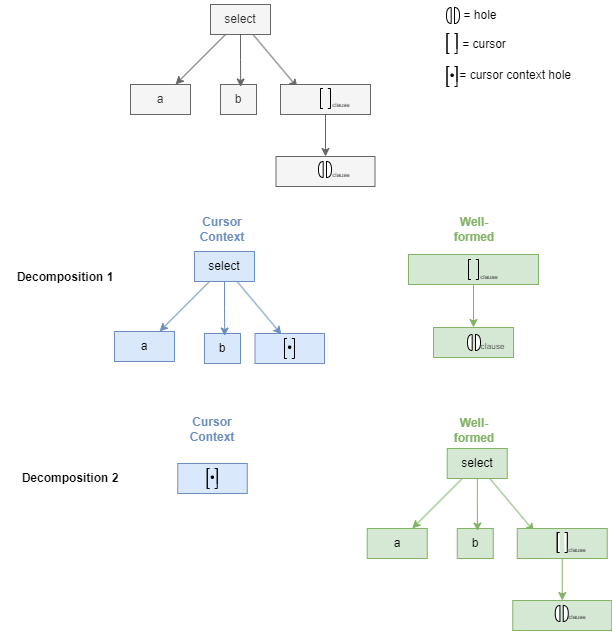
\includegraphics[width=\linewidth]{img/slq-decompose-ex.drawio.png}
  \caption{Two different decompositions of the same term}
  \label{fig:sql-decomp-ex}
\end{figure}

In order to generate a decomposition function which works for any sort,
it is necessary to specify how we for any term in any sort,
can decompose uniquely into a cursor context and well-formed-tree pair.

Unique decomposition of an \abt can be defined algorithmically and divided
into following sub-tasks:
\begin{itemize}
  \item Locate the cursor in the tree to be decomposed and generate a path to the cursor
  \item Generate an \abt of sort $s^C \in \mathcal{S}^C$ based on the cursor path
  \item Generate an \abt of sort $\dot{s} \in \dot{\mathcal{S}}$
        based on the rest of the tree that was not traversed
        when generating the cursor context
\end{itemize}

The next section will explain in more details how the steps above can be done,
and how we always get a unique decomposition, as long as the \abt to be decomposed is well-formed.

This way of decomposing an \abt always places the cursor at the root of the
well-formed tree. This makes it impossible for the cursor to encapsulate the immediate
child of the root, rendering the property of well-formed trees having a cursor at one of the immediate children of the root redundant. For this reason, the code generation
has been revised to only generate an operator of arity $(\hat{s})\dot{s}$,
representing that the cursor only encapsulates the root of a cursorless ABT
of sort $\hat{s}$.

\subsubsection{Cursor path}

Generating a path to the cursor in the \abt of sort $s \in \mathcal{S}$ extended with
hole and cursor operators simplifies the process of generating the cursor context. The path tells us
which operator $o^C \in \mathcal{O}^C$ replaces each $o \in \mathcal{O}$.
The list can be generated by performing pre-order traversal of the tree to be decomposed,
extending the list with every $i$, representing which argument in an operator of
arity $(\vec{s}_1.s_1, ... , \vec{s}_i.s_i, ..., \vec{s}_n.s_n)\mathcal{S}$ was
followed to locate the cursor. 

The implementation of such a function depends on the set of sorts $\mathcal{S}$
and arity-indexed family of operators $\mathcal{O}$ given by the abstract syntax
of a language. The Elm CodeGen package\cite{elm-codegen-package} has is used to
generate a \texttt{getCursorPath} function for a \texttt{Base} type, which returns a list of integers, indicating, form the root, which $i$ is taken for each operator $o(i_1,i_2,...,i_n) \in \mathcal{O}$ until the cursor is reached.

\subsubsection{Cursor context}

Having the cursor path, the cursor context can be generated by replacing every
operator $o \in \mathcal{O}$ with its corresponding cursor context operator
$o^C \in \mathcal{O}^C$, with respect to which argument in the operator was
followed to locate the cursor. This is also done by performing pre-order traversal
of the tree, but it will stop when the cursor is reached (i.e. when the
cursor path is empty) and replace the operator reached with the
context hole operator $[ \ \cdot \ ] \in C$. The rest of the tree which has not
been traversed will be passed to the next step, building the well-formed tree.

Functions supporting building cursor contexts are generated by Elm CodeGen, where a \texttt{toCCtx} function is generated
for the \texttt{Base} type in conjunction with a
\texttt{toCCtx\_s} for every $s$ syntactic category in the given syntax, where
the algorithm described above is implemented for every sort.

\subsubsection{Well-formed tree}

The well-formed tree is generated by performing pre-order traversal of the
rest of the tree that was not traversed when generating the cursor context.
This is done by first replacing the cursor operator $o \in \mathcal{O}$ with the well-formed operator
$\dot{o} \in \dot{\mathcal{O}}$ of arity $(\hat{s})\dot{s}$ indicating that the
cursor encapsulates a cursorless \abt of sort $\hat{s}$, being the cursorless equivalent of the child of $o$.
After this, the rest of the tree is traversed, and every operator $o \in \mathcal{O}$
is replaced with its corresponding cursorless operator $\hat{o} \in \hat{\mathcal{O}}$.

The cursor context and well-formed tree pair as defined above will decompose
any well-formed \abt into a unique pair of a cursor context and a well-formed tree.


\subsubsection{Cursor movement - Child}
Cursor movement is a fundamental operation, allowing the editor to move the cursor
to a different position, changing the target of editor expressions. This is defined
as two operations in the editor calculus in the form of
\texttt{Child-i} and \texttt{Parent} operations (\cref{fig:cursor_movement_rules}).

For moving to child $i$ of an operator, a \texttt{child} function is generated
which takes an integer $i$ and a decomposed tree represented by a tuple of a cursor
context and well-formed tree. It returns a new tuple, where the context hole in
the cursor context has been replaced with the operator of sort $\mathcal{S}^C$ corresponding to the cursorless
operator of sort $\hat{\mathcal{S}}$ under the cursor in the well-formed tree before
moving the cursor. The integer $i$ determines which argument of the cursor context
operator contains the new context hole. The new well-formed tree is built by
wrapping the $i$th argument of the cursorless operator current root operator
in the well-formed tree.

For a visualization of this, see \cref{fig:movement-example} showing the result
of applying various \texttt{child} operations to a decomposed tree.

\begin{figure}[H]
  \centering
  \begin{subfigure}[b]{0.9\linewidth}
    \centering
    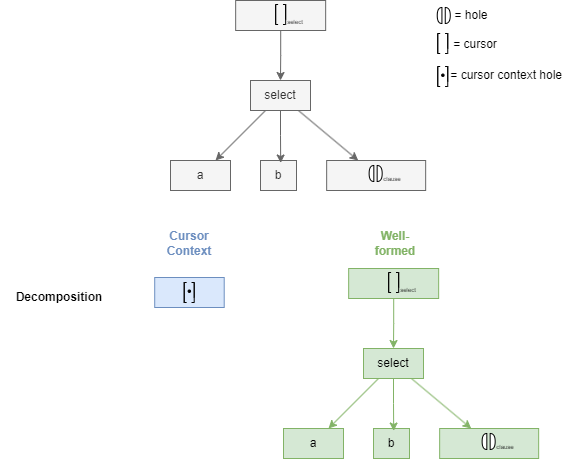
\includegraphics[width=\linewidth]{img/slq-decomp-only.drawio.png}
    \caption{Decomposition of a small SQL program}
    \label{subfig:decomp-only}
  \end{subfigure}
  \hfill
  \begin{subfigure}[b]{0.9\linewidth}
    \centering
    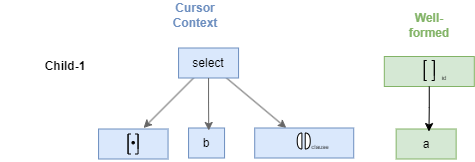
\includegraphics[width=\linewidth]{img/sql-child1.drawio.png}
    \caption{Applying the \texttt{Child-1} operation}
    \label{subfig:child1}
  \end{subfigure}
  \hfill
  \begin{subfigure}[b]{0.9\linewidth}
    \centering
    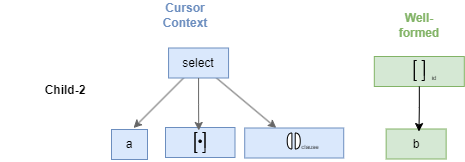
\includegraphics[width=\linewidth]{img/sql-child2.drawio.png}
    \caption{Applying the \texttt{Child-2} operation}
    \label{subfig:child2}
  \end{subfigure}
  \caption{Example of cursor movement}
  \label{fig:movement-example}
\end{figure}

This has been implemented by having Elm CodeGen generate a \texttt{child} function which
takes an integer $i$ and a decomposed tree, and returns a new cursor context
and well-formed tree pair, where the cursor has been moved to the $i$th child.

\subsubsection{Cursor movement - Parent}

Moving the cursor to the parent of the cursor is done by first updating the cursor context
by moving the context hole a level up, such that the parent of the context hole
becomes the new context hole. Then, the parent of the cursor context which has
been updated (operator of sort $\mathcal{S}^C$) is inserted as its equivalent
well-formed operator (operator of sort $\dot{\mathcal{S}}$) at the root of the
well-formed tree, where the prior root of the well-formed tree becomes an argument to the new root operator.

To visualize this, consider the example already given for the \texttt{child} operations, but where applying the \texttt{Parent} operation to the tree in \cref{subfig:child2} would result in the tree in \cref{subfig:decomp-only}.

\subsubsection{Conditional expressions, Sequence, Recursion and Context}

Conditional expressions provide a way to perform different operations based on
modal logic of the encapsulated ABT, such as the $@o$ operator which holds
if the cursor is encapsulating the operator $o$. This is defined as \texttt{At-op}
along \texttt{Necessity}, \texttt{Possibly-i} and \texttt{Possibly-i} operators
in the editor calculus (\cref{fig:satisfaction_relation_modal}). Conditionals
can be connected with logical operators, forming the operators \texttt{Negation},
\texttt{Conjunction}, \texttt{Disjunction-1} and \texttt{Disjunction-2}
(\cref{fig:satisfaction_relation_connectives}).

With the current state of the implementation, it is only possible to query for a given conditional expression $\phi$, which will return wether that condtion holds. The rest is yet to be implemented.

\subsubsection{Generic implementation}
Given the generic nature of the editor calculus, the implementation could
benefit from type classes, which would allow for more general functions
to be written, without the need for explicit references to specific
function implementations for different sorts.

For example, consider the cursor substitution operator
(\cref{fig:substitution_rules}), where the editor calculus enforces
that operators can only be substituted with operators of same
sort. Initially, a straightforward approach involves having a
substitution function for each sort $s \in \mathcal{S}$.  This
approach of course leads an implementer to consider generalization,
i.e. how a single function can take any cursor-encapsulated \abt and
replace it with an operator of the same sort. A solution to this could
be using type classes, where we might have a type class called
\texttt{substitutable} and having an instance for each sort.  This is
not directly supported Elm but in Haskell; we would then use the
solution shown in \cref{lst:haskell-typeclass}.  Typeclasses can
however be simulated with Elm records, as shown in the "typeclasses"
Elm package\cite{elm-typeclass-package}.  An example of this is shown
in \cref{lst:elm-typeclass}.  This approach has the disadvantage of
forcing an explicit reference to the typeclass "instance" in a generic
function, in contrast to Haskell.

% TODO: replace this with a more interesting example, i.e. conditionals
\begin{lstlisting}[language=Haskell,style=inline,caption={Haskell typeclass example},label={lst:haskell-typeclass}]
class Substitutable a where 
    substitute :: a -> a -> a
    
instance Substitutable a where
    substitute _ replacement = replacement

doIntSub :: Int
doIntSub = substitute 1 2 
\end{lstlisting}

\begin{lstlisting}[language=elm,style=inline,caption={Elm typeclass simulation example},label={lst:elm-typeclass}]
type alias Substitutable a =
    { substitute : a -> a -> a }

substituteAny : Substitutable a
substituteAny =
    { substitute = \_ replacement -> replacement }

substitute : Substitutable a -> a -> a -> a
substitute substitutable expression replacement =
    substitutable.substitute expression replacement

doIntSub : Int
doIntSub =
    substitute substituteAny 1 2
\end{lstlisting}

Unfortunately, this leads to more verbose code and it does not solve the rigid source code generation, since direct references to the typeclass "instance" is needed, which are made out of manipulated strings (although with assistance from the Elm CodeGen package). In other words, this
does not provide any benefits over referring to a concrete function for
each sort, which is the current approach.

\section{Conclusion and Further Work}

We have developed a generalized editor calculus that enables the
creation of a syntax-directed editor calculus for a specific abstract
syntax, and describe how to encode it into a monomorphic typed lambda
calculus with pairs, recursion and pattern matching. The encoding is
sound, and as a consequence, given that the type system of the
extended lambda calculus is sound, it follows that our editor calculus
is typesafe.

Further work on our generalized editor calculus is to prove whether
the encoding is complete.  A next, important next step is to
incorporate a copy-paste operation since this is a central notion in
editing. Here, the question arises as to how to best deal with pasting
terms that include free variables. In some settings, when editing
code, this will introduce name clashes, but in other settings the free
variables should intentionally be captured. A likely solution is
therefore to have two different paste operations corresponding to each
of these situations.

\bibliographystyle{ACM-Reference-Format}
\bibliography{bibliography}


\end{document}
\endinput

%%% Local Variables:
%%% mode: latex
%%% TeX-master: t
%%% End:
